% ----------------------------------------------------------
\chapter{Resultados}
% ----------------------------------------------------------
\section{Hospedagem e Pubicação}

O WebBalmy.jl foi publicado utilizando o GitHub Pages, uma ferramenta gratuita para serviços fornecidos por APIs. Ele hospeda sites estáticos criados a partir de repositórios Git, um sistema de controle de versões distribuído, usado principalmente no desenvolvimento de \textit{software}, pois salva todo o histórico de edições contido no processo de construção de um programa computacional. 

\section{Interface gráfica}

\section{Representação tridimensional}
Para representar os modelos tridimensionais utilizando o Three.js, é utilizado o modelo de Blinn-Phong, capaz de simular superfícies brilhantes com holofotes especulares. O sombreamento é calculado \textit{per pixel} de acordo com o modelo de Phong. Desse modo, apesar de custar um pouco mais de tempo para renderizar, ele atinge uma acurácia maior do que outros modelos disponíveis (o de Lambert, por exemplo).

No modelo primeiramente proposto por Phong, é calculado continuamente o produto escalar $R \cdot V$ entre um observador $V$ e o feixe de uma fonte de luz ($L$) refletida ($R$) sobre uma superfície. No ajuste proposto por Blinn, no entanto, calcula-se um vetor a meio caminho entre o espectador e os vetores de fonte luminosa, podendo substituir $R \cdot V$ por $N \cdot H$, onde $N$ é o vetor normal ã superfície.

\begin{figure}[htb]
\begin{equation}
    \label{eq:R1}
    H = \frac{L + \highlight{blue}{V} }{||L + \tikzmarknode{value}{\highlight{blue}{V}}||}
\end{equation}
\begin{tikzpicture}[overlay,remember picture,>=stealth,nodes={align=left,inner ysep=1pt},<-]
    \path (value.south) ++ (-1,-1.5em) node[anchor=north east,color=blue!67] (scalep){\textit{$V = P_H (-L)$}};
    \draw [color=blue!87](value.south) |- ([xshift=-1.65em,color=blue]scalep.north west);
\end{tikzpicture}
\vspace{2\baselineskip}
\end{figure}

Na \autoref{eq:R1}, $P_H$ é a matriz de Householder que reflete um ponto no hiperplano que contém a origem e tem um vetor normal $H$. Este produto escalar é o cosseno de um ângulo que é metade do ângulo representado pelo produto escalar de Phong (se $V$, $L$, $N$ e $R$ estiverem todos no mesmo plano). Esta relação entre os ângulos sofre desvios discretos quando os vetores não se encontram no mesmo plano, especialmente em relação aos ângulos pequenos.

Ainda sobre os ajustes de Blinn ao modelo de Phong, consideremos que o ângulo entre o vetor a meio caminho $(N \cdot H)$ e a superfície normal é provavelmente menor do que o ângulo entre $R$ e $V$ usado no modelo original (a menos que a superfície seja vista de um ângulo muito íngreme para o qual é provável que seja maior), e já que Phong está usando $(R \cdot V)^\alpha$, um expoente (chamado de constante de brilho) pode ser definido como $\alpha' > \alpha$, tal que $(N \cdot H)^{\alpha'}$ está mais próxima da expressão original de Phong.

\begin{figure}[htb]
\caption{\label{fig:representations} Exemplo da aplicação do modelo de Blinn-Phong na molécula de benzenos a partir da alteração dos coeficientes $\alpha'$ para os átomos (representados por esferas). Da direita para a esquerda, os valores atribuídos foram: 0, 10, 50, 100, 1000; respectivamente.}
	\begin{center}
		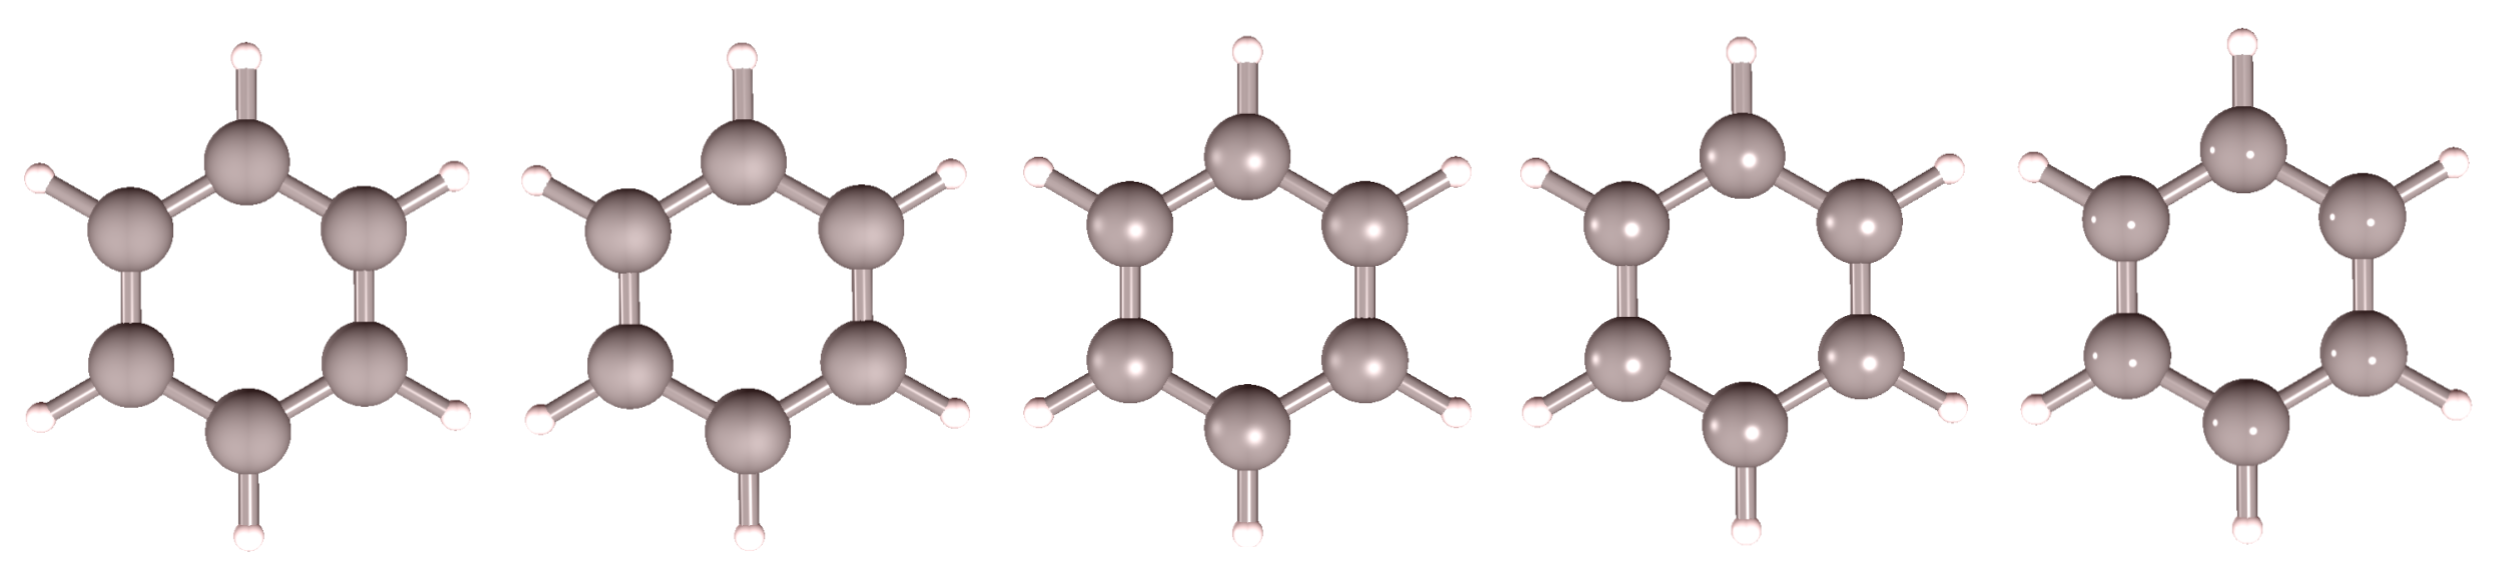
\includegraphics[width=1.0\textwidth]{images/shininess(1).png}
	\end{center}
	\fonte{Autor(a)}
\end{figure}

Variando, portanto, o valor de $\alpha'$, é possível notar que, na \autoref{fig:representations}, quanto maior for seu valor, menor será o holofote especular, representado pelos pontos luminosos nas estruturas moleculares.

\section{Influência de K}

\section{Diagramas de orbitais moleculares}

\section{Otimização de geometria}

\section{Índices geométricos}

\begin{figure}[htb!]
    \centering
    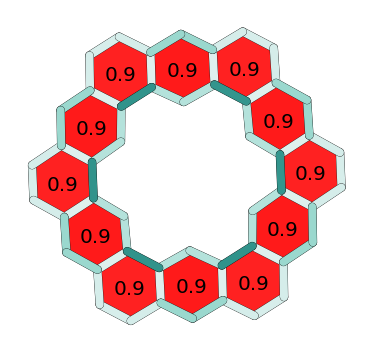
\includegraphics[width=0.36\textwidth]{images/kekulene.png}
    \caption{Caption}
    \label{fig:my_label}
\end{figure}

\begin{figure}[htb!]
    \centering
    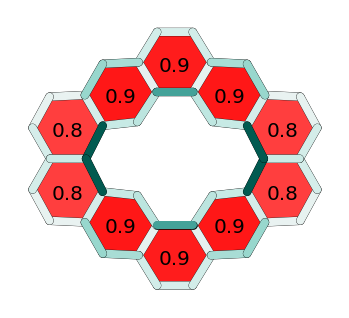
\includegraphics[width=0.36\textwidth]{images/Icosaene.png}
    \caption{Caption}
    \label{fig:my_label}
\end{figure}

\begin{figure}[htb!]
    \centering
    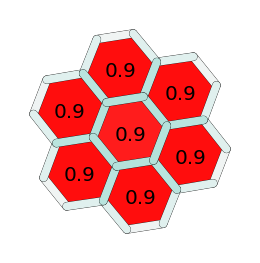
\includegraphics[width=0.28\textwidth]{images/coronene.png}
    \caption{Caption}
    \label{fig:my_label}
\end{figure}

\begin{figure}[htb!]
    \centering
    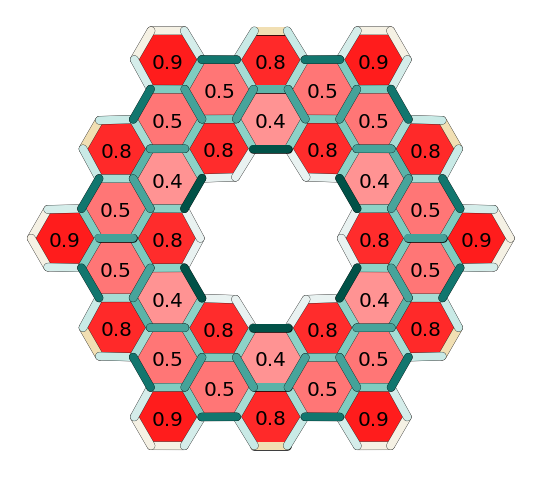
\includegraphics[width=0.6\textwidth]{images/output.png}
    \caption{Caption}
    \label{fig:my_label}
\end{figure}